\documentclass[12pt, a4paper]{article}
\usepackage[utf8]{inputenc}
\usepackage[russian]{babel}
\usepackage[pdftex]{graphicx, color}
\usepackage{amsmath}
\usepackage{amsfonts}
\usepackage{amssymb}
\usepackage{amsthm}
\usepackage[left=2cm,right=1.5cm,top=1.5cm,bottom=2cm]{geometry}
\usepackage{indentfirst}
\usepackage{hyperref}

\usepackage{pbox}

\usepackage{setspace}
\onehalfspacing
\graphicspath{{pic/}}

\begin{document}

    \thispagestyle{empty}

    \begin{singlespace}
    \begin{titlepage}
        \begin{center}
            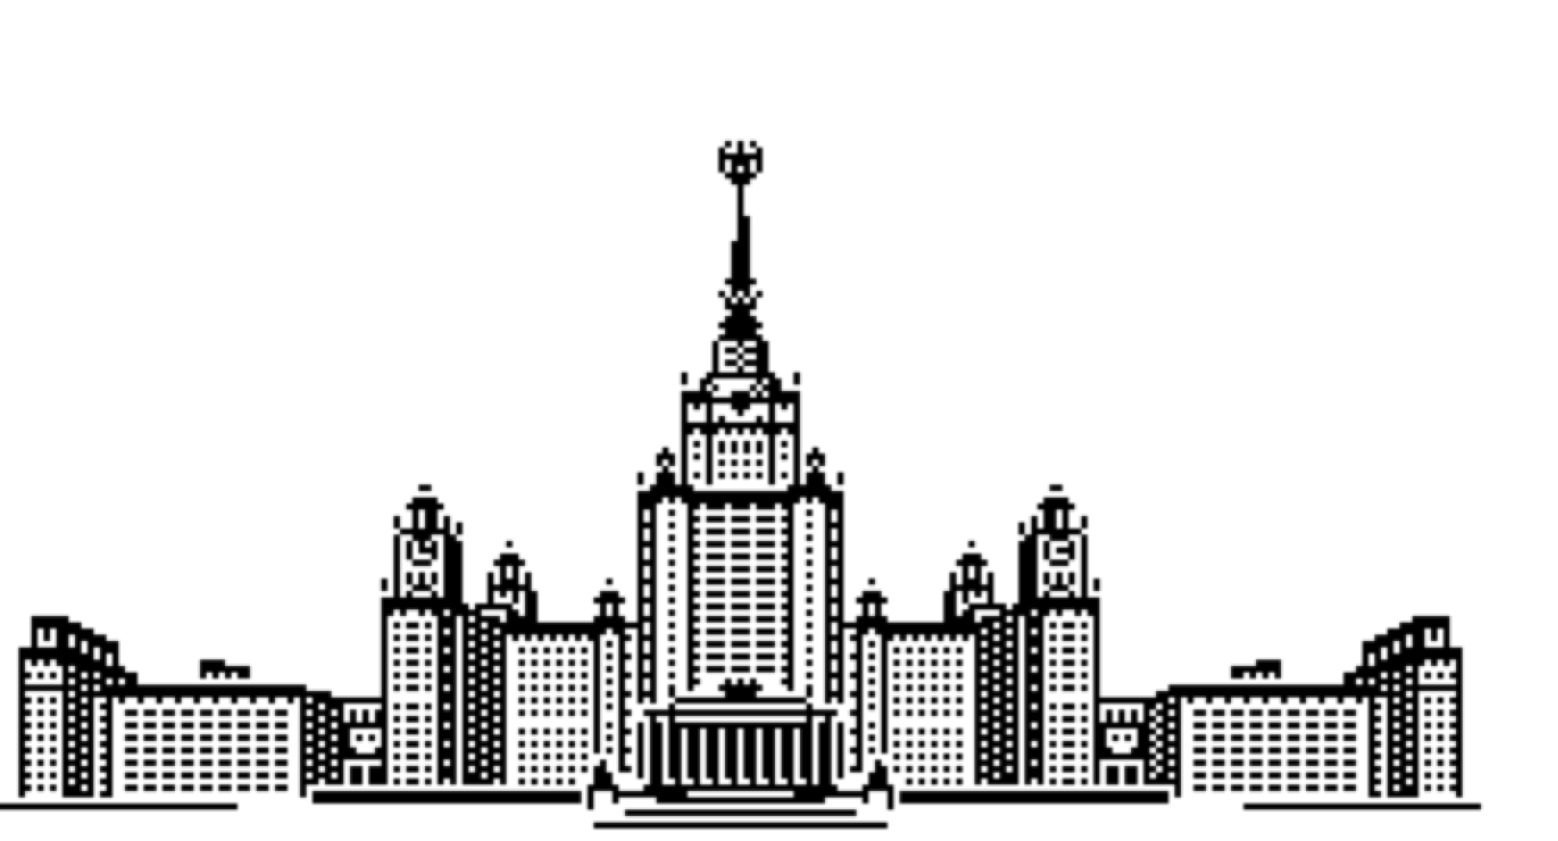
\includegraphics[height = 3cm]{msu.png}

            {\scshape Московский государственный университет имени М.~В.~Ломоносова}\\
            Факультет вычислительной математики и кибернетики\\
            \centerline{\hfill\hrulefill\hrulefill\hrulefill\hrulefill\hfill}

            \vfill

            {\LARGE Отчет к Лабораторной работе \textnumero2: \\ Изучение и освоение методов анализа формы объектов в изображениях}

            \vspace{1cm}

        \end{center}

        \vfill
        \begin{flushright}
            \textit{Студент 3 курса ВМК (317 группа):}\\
                Оспанов А.М.

            \vspace{5mm}

        \end{flushright}

        \vfill

        \begin{center}
        Москва, 2015
        \end{center}
    \end{titlepage}
    \end{singlespace}

    \tableofcontents

    \newpage
    \section{Введение}
        Данный отчет был написан по дисциплине ``Обработка и распознавание изображений'' студентом 317 группы Оспановым Аятом.

        В данной работе нужно было реализовать алгоритм для подсчета количества столовых приборов на изображении. Для этого использовалась сегментация изображений в виде бинарного изображения на основе точечных, пространственных и морфологических преобразований. В качестве языка программирования использовался Python версии 2 с библиотекой skimage.

    \newpage
    \section{Основная часть}
        \subsection{Исследование изображений}

            Как и в любой работе по распознаванию изображений, все началось с бинаризации. Но тут же мы сталкиваемся с проблемой - с проблемой вспышки. При съемке столовых приборов использовалась вспышка, что усложнило задачу, т.к. яркость на изображении прыгает в зависимости от изгиба приборов и появляются блики. Но немножко посмотрев на изображения, было замечено, что бинаризация хорошо работает на красном канале изображения, нежели на gray-scale. Поэтому был взят красный канал изображения.

            \begin{center}
                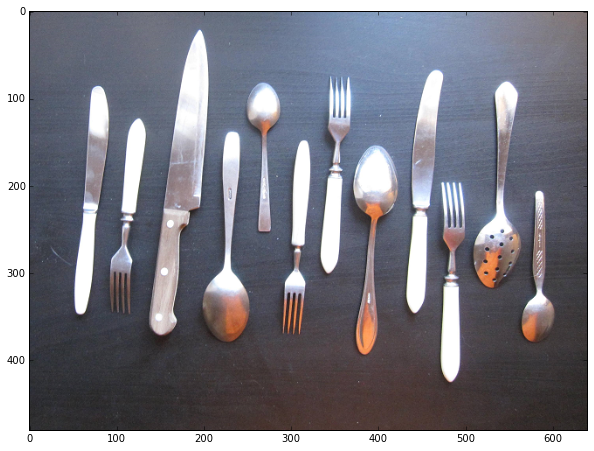
\includegraphics[width=10cm]{0.png}
            \end{center}

            Далее были проведены:

            1) морфологическая операция эрозия. Ядро - круг с радиусом 1. Это было сделано для зубцов вилок, чтобы они утончались, тем самым увеличивая расстояние между ними.

            \begin{center}
                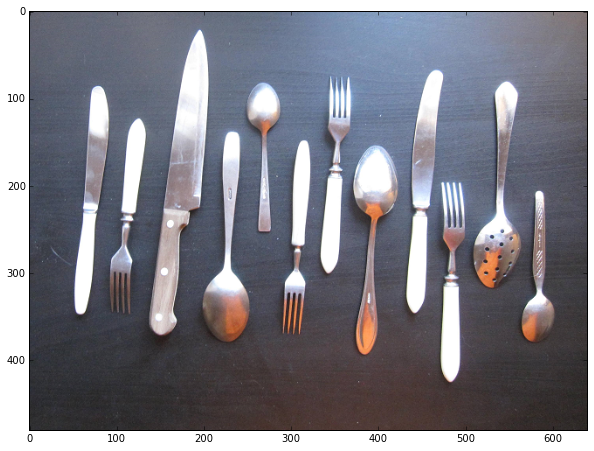
\includegraphics[width=10cm]{1.png}
            \end{center}

            2) адаптивная нормализация контраста
            \begin{center}
                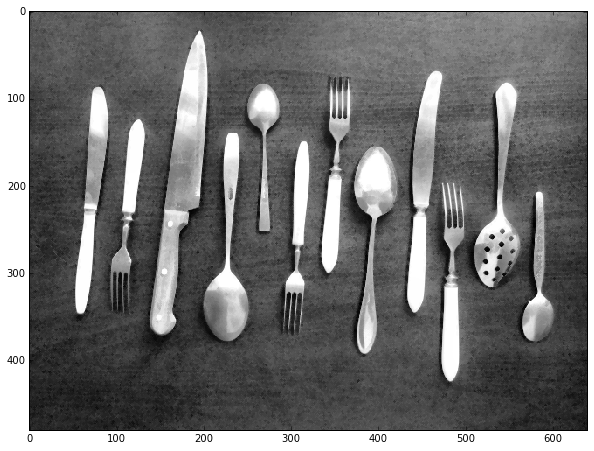
\includegraphics[width=10cm]{2.png}
            \end{center}

            3) фильтр Собеля для нахождения границы
            \begin{center}
                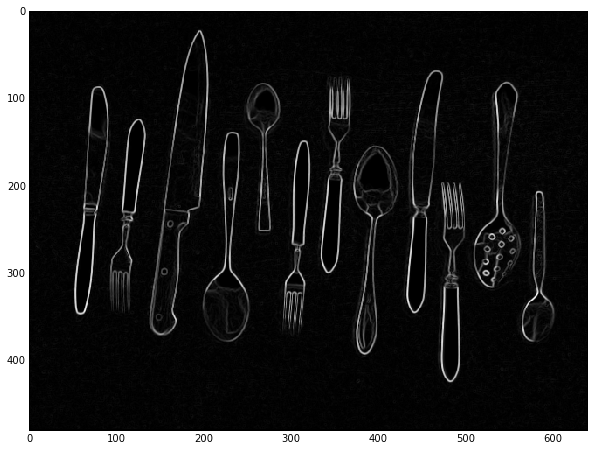
\includegraphics[width=10cm]{3.png}
            \end{center}

            4) бинаризация адаптивным методом (метод локального порога с ядром Гаусса)
            \begin{center}
                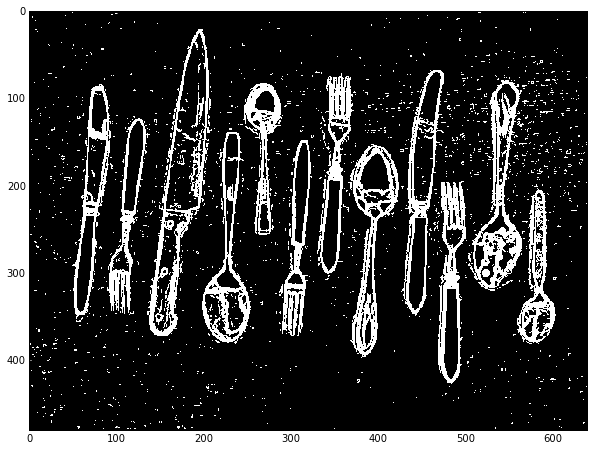
\includegraphics[width=10cm]{4.png}
            \end{center}

            5) убирались мелкие компоненты
            \begin{center}
                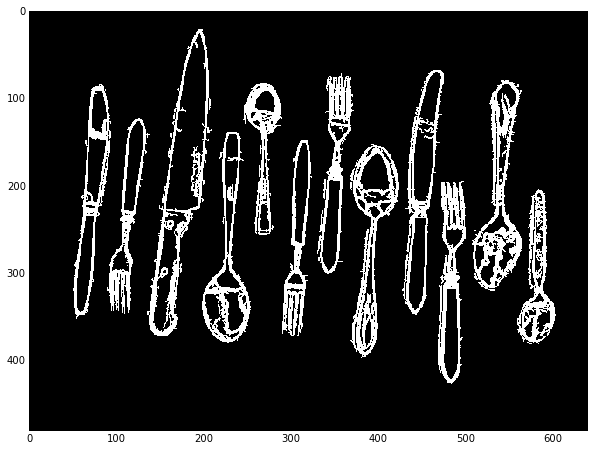
\includegraphics[width=10cm]{5.png}
            \end{center}

            6) заполнялись замкнутые области
            \begin{center}
                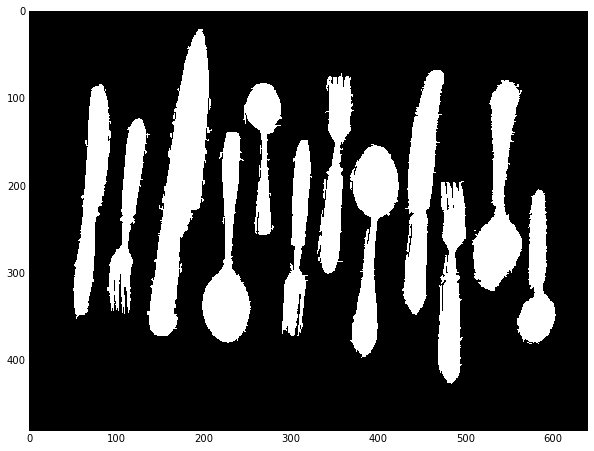
\includegraphics[width=10cm]{6.png}
            \end{center}

            7) эрозия + убирались мелкие компоненты для удаления мелких выступов
            \begin{center}
                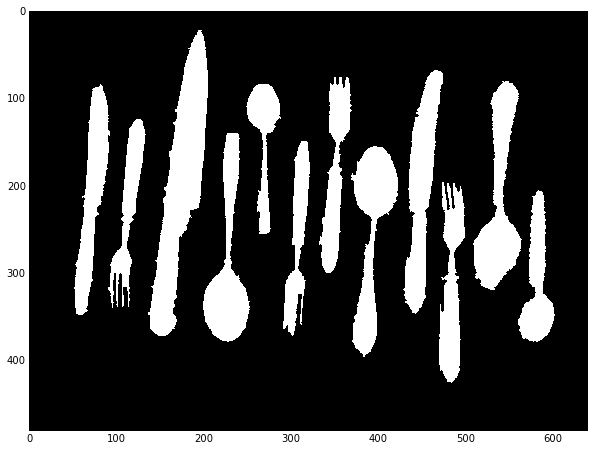
\includegraphics[width=10cm]{7.png}
            \end{center}

            8) назначались метки
            \begin{center}
                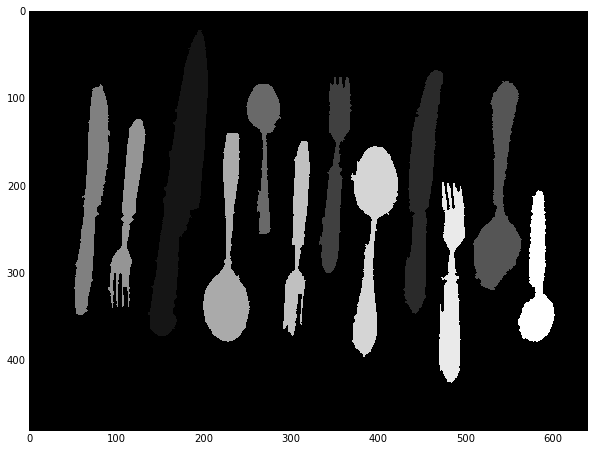
\includegraphics[width=10cm]{8.png}
            \end{center}

            9) сама классификация:
            \begin{itemize}
                \item вычислялась компактность: у вилки интервал значений компактностей лежал вне интервалов компактностей ложек и ножей, тем самым удалось выделить вилки
                \item но интервалы компактностей ложек и ножей пересекались, т.о. нам нужно провести морфологические преобразования. Для этого было решено провести дилатацию большим кругом, тем самым оставив только овальную часть ложки и удалив все или оставив тонкую линию в случае ножей. Теперь ложка легко отделялась от ножа.
            \end{itemize}

            В итоге получаем результат
            \begin{center}
                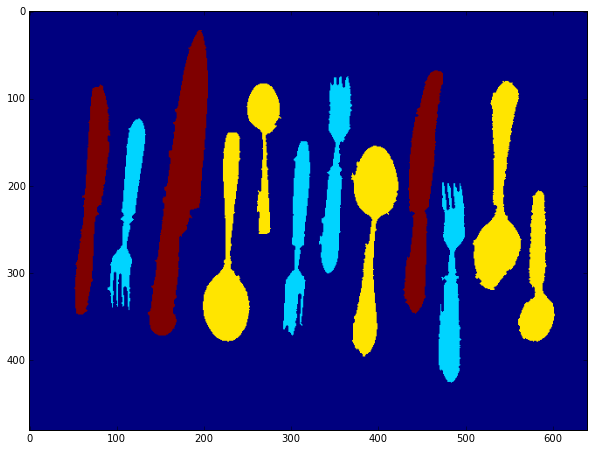
\includegraphics[width=10cm]{9.png}
            \end{center}


    \newpage
    \section{Заключение}

        Данный алгоритм сработал на 1 и 2 изображениях. Результаты можно увидеть в следующей таблице:

        \begin{center}
        \begin{tabular}{c c}
            {\bf Исходное изображение} & {\bf Конечное изображение} \\
            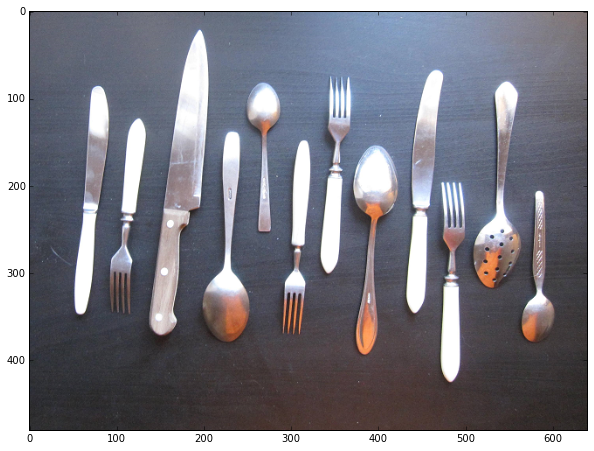
\includegraphics[width=8cm]{0.png} & 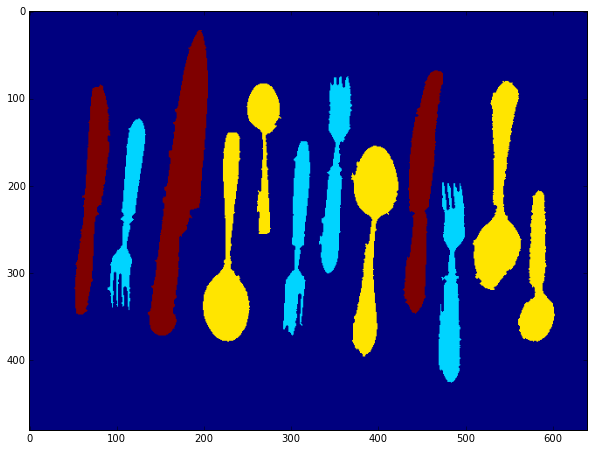
\includegraphics[width=8cm]{9.png} \\
            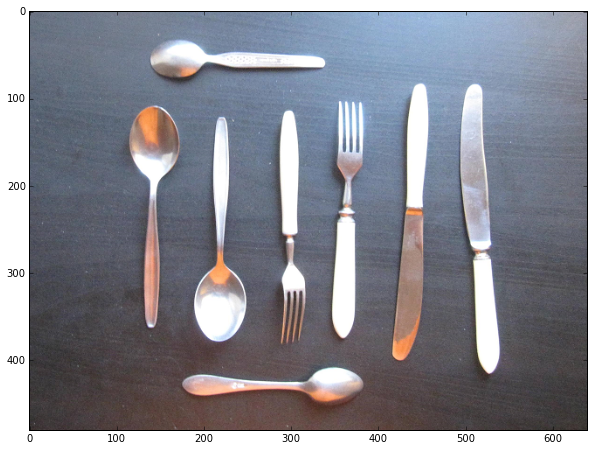
\includegraphics[width=8cm]{00.png} & 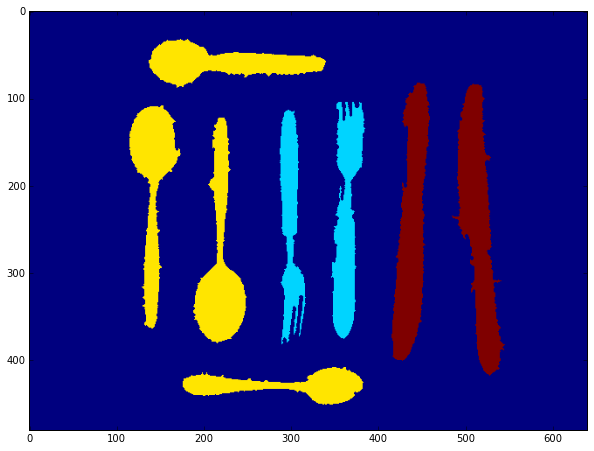
\includegraphics[width=8cm]{99.png} \\
        \end{tabular}
        \end{center}

        На других изображения алгоритм не сработал, т.к. либо при бинаризации и заполнении полостей несколько приборов соединялись, либо зубцы вилок заполнялись и не отличались от других приборов.

        \begin{center}
        \begin{tabular}{c c}
            {\bf Случай соединения приборов} & {\bf Случай заполнения зубцов вилок} \\
            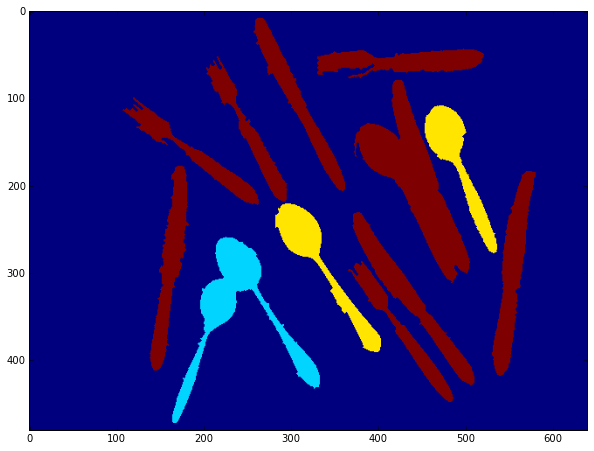
\includegraphics[width=8cm]{err1.png} & 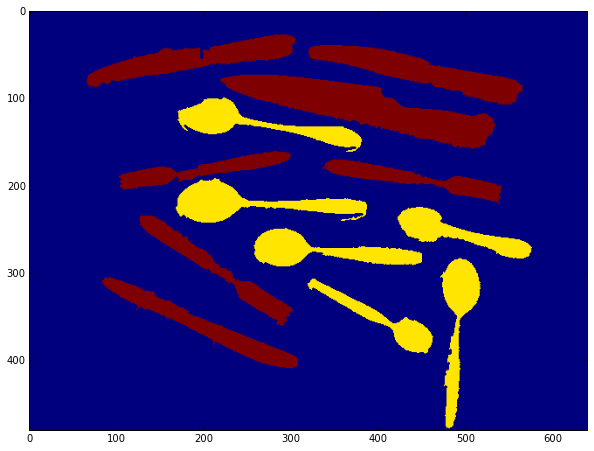
\includegraphics[width=8cm]{err2.png} \\
        \end{tabular}
        \end{center}

        
\end{document}
